\documentclass{article}
%----------------------------------------------------------------------------------------
%	PACKAGES AND OTHER DOCUMENT CONFIGURATIONS
%----------------------------------------------------------------------------------------

\usepackage{amsmath,amsfonts,stmaryrd,amssymb} % Math packages

\usepackage{enumerate} % Custom item numbers for enumerations
\usepackage{tikz}
\usetikzlibrary{arrows}
\usepackage[ruled]{algorithm2e} % Algorithms

\usepackage[framemethod=tikz]{mdframed} % Allows defining custom boxed/framed environments

\usepackage{listings} % File listings, with syntax highlighting
\lstset{
	basicstyle=\ttfamily, % Typeset listings in monospace font
}

%----------------------------------------------------------------------------------------
%	DOCUMENT MARGINS
%----------------------------------------------------------------------------------------

\usepackage{geometry} % Required for adjusting page dimensions and margins
\usepackage{graphicx, amsmath, amsthm, amssymb, listings, multirow, wrapfig, floatrow}
\newcommand{\bigCI}{\mathrel{\text{\scalebox{1.07}{$\perp\mkern-10mu\perp$}}}}
\usepackage{xepersian}
\settextfont[Scale=1]{XB Niloofar}
\setdigitfont[Scale=1]{Yas}

\geometry{
	paper=a4paper, % Paper size, change to letterpaper for US letter size
	top=2.5cm, % Top margin
	bottom=3cm, % Bottom margin
	left=2.5cm, % Left margin
	right=2.5cm, % Right margin
	headheight=14pt, % Header height
	footskip=1.5cm, % Space from the bottom margin to the baseline of the footer
	headsep=1.2cm, % Space from the top margin to the baseline of the header
	%showframe, % Uncomment to show how the type block is set on the page
}

%----------------------------------------------------------------------------------------
%	COMMAND LINE ENVIRONMENT
%----------------------------------------------------------------------------------------

% Usage:
% \begin{commandline}
%	\begin{verbatim}
%		$ ls
%		
%		Applications	Desktop	...
%	\end{verbatim}
% \end{commandline}

\mdfdefinestyle{commandline}{
	leftmargin=10pt,
	rightmargin=10pt,
	innerleftmargin=15pt,
	middlelinecolor=black!50!white,
	middlelinewidth=2pt,
	frametitlerule=false,
	backgroundcolor=black!5!white,
	frametitle={Command Line},
	frametitlefont={\normalfont\sffamily\color{white}\hspace{-1em}},
	frametitlebackgroundcolor=black!50!white,
	nobreak,
}

% Define a custom environment for command-line snapshots
\newenvironment{commandline}{
	\medskip
	\begin{mdframed}[style=commandline]
}{
	\end{mdframed}
	\medskip
}

%----------------------------------------------------------------------------------------
%	FILE CONTENTS ENVIRONMENT
%----------------------------------------------------------------------------------------

% Usage:
% \begin{file}[optional filename, defaults to "File"]
%	File contents, for example, with a listings environment
% \end{file}

\mdfdefinestyle{file}{
	innertopmargin=1.6\baselineskip,
	innerbottommargin=0.8\baselineskip,
	topline=false, bottomline=false,
	leftline=false, rightline=false,
	leftmargin=2cm,
	rightmargin=2cm,
	singleextra={%
		\draw[fill=black!10!white](P)++(0,-1.2em)rectangle(P-|O);
		\node[anchor=north west]
		at(P-|O){\ttfamily\mdfilename};
		%
		\def\l{3em}
		\draw(O-|P)++(-\l,0)--++(\l,\l)--(P)--(P-|O)--(O)--cycle;
		\draw(O-|P)++(-\l,0)--++(0,\l)--++(\l,0);
	},
	nobreak,
}

% Define a custom environment for file contents
\newenvironment{file}[1][File]{ % Set the default filename to "File"
	\medskip
	\newcommand{\mdfilename}{#1}
	\begin{mdframed}[style=file]
}{
	\end{mdframed}
	\medskip
}

%----------------------------------------------------------------------------------------
%	NUMBERED QUESTIONS ENVIRONMENT
%----------------------------------------------------------------------------------------

% Usage:
% \begin{question}[optional title]
%	Question contents
% \end{question}

\mdfdefinestyle{question}{
	innertopmargin=1.2\baselineskip,
	innerbottommargin=0.8\baselineskip,
	roundcorner=5pt,
	nobreak,
	singleextra={%
		\draw(P-|O)node[xshift=1em,anchor=west,fill=white,draw,rounded corners=5pt]{%
		Question \theQuestion\questionTitle};
	},
}

\newcounter{Question} % Stores the current question number that gets iterated with each new question

% Define a custom environment for numbered questions
\newenvironment{question}[1][\unskip]{
	\bigskip
	\stepcounter{Question}
	\newcommand{\questionTitle}{~#1}
	\begin{mdframed}[style=question]
}{
	\end{mdframed}
	\medskip
}

%----------------------------------------------------------------------------------------
%	WARNING TEXT ENVIRONMENT
%----------------------------------------------------------------------------------------

% Usage:
% \begin{warn}[optional title, defaults to "Warning:"]
%	Contents
% \end{warn}

\mdfdefinestyle{warning}{
	topline=false, bottomline=false,
	leftline=false, rightline=false,
	nobreak,
	singleextra={%
		\draw(P-|O)++(-0.5em,0)node(tmp1){};
		\draw(P-|O)++(0.5em,0)node(tmp2){};
		\fill[black,rotate around={45:(P-|O)}](tmp1)rectangle(tmp2);
		\node at(P-|O){\color{white}\scriptsize\bf !};
		\draw[very thick](P-|O)++(0,-1em)--(O);%--(O-|P);
	}
}

% Define a custom environment for warning text
\newenvironment{warn}[1][Warning:]{ % Set the default warning to "Warning:"
	\medskip
	\begin{mdframed}[style=warning]
		\noindent{\textbf{#1}}
}{
	\end{mdframed}
}

%----------------------------------------------------------------------------------------
%	INFORMATION ENVIRONMENT
%----------------------------------------------------------------------------------------

% Usage:
% \begin{info}[optional title, defaults to "Info:"]
% 	contents
% 	\end{info}

\mdfdefinestyle{info}{%
	topline=false, bottomline=false,
	leftline=false, rightline=false,
	nobreak,
	singleextra={%
		\fill[black](P-|O)circle[radius=0.4em];
		\node at(P-|O){\color{white}\scriptsize\bf i};
		\draw[very thick](P-|O)++(0,-0.8em)--(O);%--(O-|P);
	}
}

% Define a custom environment for information
\newenvironment{info}[1][Info:]{ % Set the default title to "Info:"
	\medskip
	\begin{mdframed}[style=info]
		\noindent{\textbf{#1}}
}{
	\end{mdframed}
}
 
\title{تمرین کامپیوتری اوّل - استنتاج علّی} 
\author{بهراد منیری\\95109564\\ \texttt{bemoniri@live.com}}
\date{دانشکده‌ی مهندسی برق - دانشگاه صنعتی شریف}
%----------------------------------------------------------------------------------------

\begin{document}
\maketitle
\section{سوال اول}
\subsection{بخش الف}	
\begin{itemize}
\item 	(\textbf{مدل خطی با نویز گاوسی})
در این مدل داریم:
$$
X \rightarrow Y :
\begin{cases}
X := N_x\\
Y := X + N 
\end{cases}
N \bigCI N_x
$$
فرض کنید
$N_x : \textrm{Normal}(0, \frac{1}{2})$
و
$ N = \textrm{Normal}(0, \frac{1}{2})$.
با این فرض، هر ترکیب خطی $X$ و $Y$ نرمال است، در نتیجه آنها مشترکاً نرمال هستند.
$$\forall \alpha, \beta: \;\;  \alpha X + \beta Y = \textrm{Normal} \rightarrow (X, Y): \textrm{Normal\;Multivariable}(0,0;1,\frac{1}{\sqrt{2}};\frac{1}{\sqrt{2}})$$

توزیع‌های شرطی یک توزیع مشترکاً نرمال نرمال است.
$$
\begin{cases}
P(Y|X=x) = \textrm{Normal}(x, \frac{1}{2})\\ 
P(X|Y=y) = \textrm{Normal}(-\frac{y}{2}, \frac{1}{2\sqrt{2}})
\end{cases}
$$
شکل
\eqref{1}
نمودار توزیع‌های مطرح شده هستند.

\begin{figure}[h!]
\centering
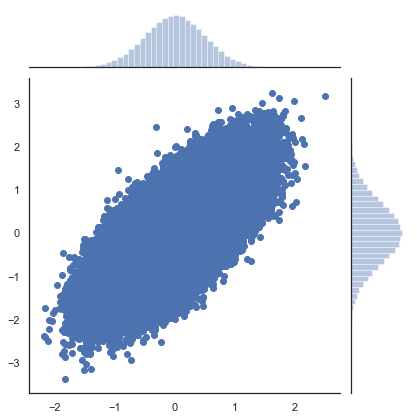
\includegraphics[scale=0.3]{lin_cond1.png}
\begin{floatrow}

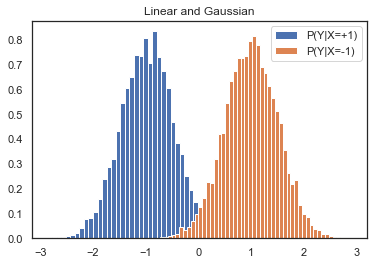
\includegraphics[scale=0.3]{lin_cond2.png}
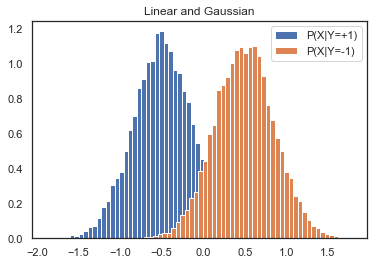
\includegraphics[scale=0.3]{lin_cond3.png}
\end{floatrow}
\caption{توزیع‌ها با فرض 	$\sigma_x = \sigma_N = 0.5$	}
\label{1}
\end{figure}


\item 	(\textbf{مدل غیرخطی با نویز گاوسی})
در این مدل داریم:
$$
X \rightarrow Y :
\begin{cases}
X := N_x\\
Y := X + 5X^3 + N 
\end{cases}
N \bigCI N_x
$$
شکل \eqref{2} نمودارهای خواسته شده‌ی مربوط به این $SCM$ با فرض
 $$N_x = \mathrm{Normal}(0, 1) \;\;\;\; N = \mathrm{Normal}(0, 10) $$
 است.

\begin{figure}[h]
\centering
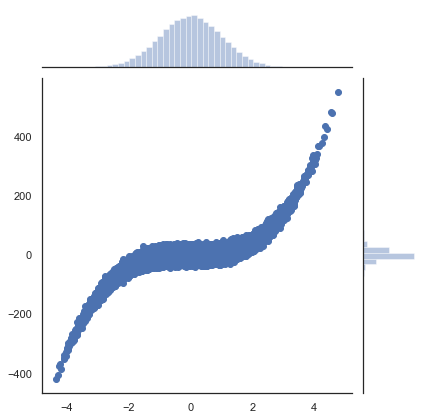
\includegraphics[scale=0.35]{non_con1.png}
\begin{floatrow}
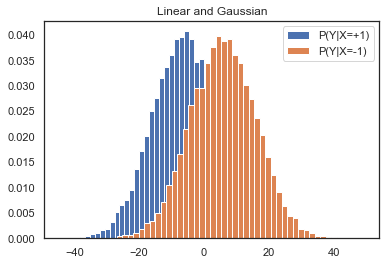
\includegraphics[scale=0.35]{non_cond2.png}
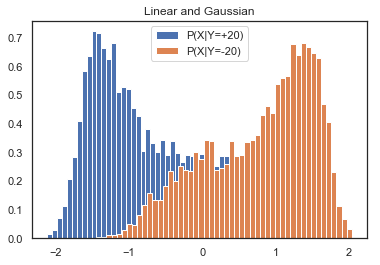
\includegraphics[scale=0.35]{non_cond3.png}
\end{floatrow}
\caption{توزیع‌ها با فرض 	
$\sigma_x =1,\;\; \sigma_N = 10$}
\label{2}
\end{figure}
\end{itemize}


\newpage
\subsection{بخش ب}
در این بخش می‌خواهیم تاثیر خطی و یا گاوسی بودن مدل را در تشخیص جهت درست علیَت  بررسی کنیم. 

\begin{itemize}
\item \textbf{بررسی اثر خطی‌بودن} 
برای بررسی اثرات غیرخطی بودن مدل، $b$ را در بازه‌ی $[-1, 1]$ تغییر می‌دهیم.  نویز مدل را گاوسی
($q=1$)
در نظر می‌گیریم.  برای مقدار مختلف $b$، در دو جهت رگرسیون انجام می‌دهیم و سپس استقلال Residue از علّت را بررسی می‌کنیم. در این تمرین، معیار ما برای استقلال، آزمون HSIC با سطح اطمینان ۲ درصد است.
برای هر $b$، صد این کار را تکرار می‌کنیم و نمودار درصد پذیرش فرض استقلال بر حسب $b$ را رسم می‌کنیم.
شکل
\eqref{nonlin}
نمایش‌دهنده‌ی نتایج ماست.
\begin{figure}[h!]
	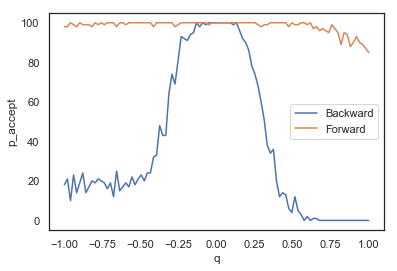
\includegraphics[scale=0.45]{nonlin.png}
	\caption{بررسی اثر خطی بودن بر تشخیص جهت علیّت}
	\label{nonlin}
\end{figure}


این نتایج با انتظارات ما کاملاً هم‌خوانی دارند زیرا در حالت خطی، و با توجه به گاوسی بودن $N$ و $X$ انتظار داریم در تشخیص جهت علیّت دچار اشتباه شویم (در مدل خطی-گاوسی، با روش مطرح شده نمی‌توان جهت را تشخیص داد و هر دو جهت ویژگی استقلال را دارا می‌باشند.)

\item \textbf{بررسی اثر گاوسی بودن} 
برای بررسی تاثیر گاوسی بودن نویز، مدل را خطی فرض کرده 
($b=0$)
و مقدار q را در بازه‌ی 
$[0.5, 2]$
تغییر می‌دهیم. مشابه بخش قبل، این بار برای مقادیر مختلف $q$، در دو جهت رگرسیون انجام داده و نمودار درصد پذیرش فرض استقلال بر حسب $q$ را رسم می‌کنیم. شکل
\eqref{gauss}
را ببینید.
\begin{figure}[h!]
	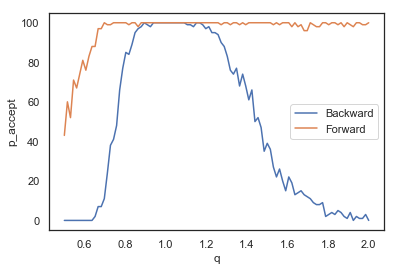
\includegraphics[scale=0.45]{gauss.png}
	\caption{بررسی اثر گاوسی بودن بر تشخیص جهت علیّت}
	\label{gauss}
\end{figure}


نتایج با انتظارت هم‌خوانی دارند زیرا طبق آنچه در کلاس بررسی کردیم، در حالت خطی-گاوسی، می‌توان SCM را، بدون بر هم خوردن شرط استقلال در هر دو جهت نوشت.
\end{itemize}
	
	
	
	
\newpage
\subsection{بخش ج}
\subsubsection{دیتاست آبفشان}

ابتدا داده‌ها را در یک فضای دو‌بعدی رسم می‌کنیم تا شهود بهتری نسبت به مسأله پیدا کنیم، شکل \eqref{abfeshan}.
\begin{figure}[h]
\centering
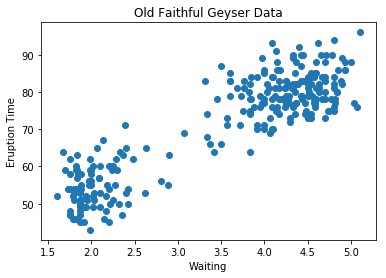
\includegraphics[scale=0.45]{old1.png}
\caption{رسم دیتای مربوط به آبفشان}
\label{abfeshan}
\end{figure}

برای تشخیص جهت درست علّیت،  با فرض \lr{ANM}، مطابق بخش‌های قبل یک‌بار هر یکی از دو متغیّر را علّت فرض کرده و رگرسیون‌های غیرخطی مربوط را انجام می‌دهیم.  
$$
\begin{cases}
Y = \hat{f_1}(X) + \hat{N}_1 &\;  :X \rightarrow Y \text{با فرض}  \\
X = \hat{f_2}(Y) + \hat{N}_2 &\;  :Y \rightarrow X \text{با فرض}
\end{cases}
$$
انتظار داریم که در جهت درست علّیت، N و متغیّری که عنوان علّت در نظر گرفته‌ایم مستقل شوند. با انجام این فرآیند در هر دو جهت و اعمال آزمون استقلال هیلبرت-اشمیت برای دو کمیت مذکور در هر جهت، جهت درست علّیت را تشخیص می‌دهیم.

شکل \eqref{erup} رگرسیون با فرض اینکه زمان فوران کنونی علّت فاصله‌ی زمانی تا فوران بعدی است و شکل \eqref{wait} نیز رگرسیون با فرض معکوس است.
\begin{figure}[h]
\begin{floatrow}
\centering
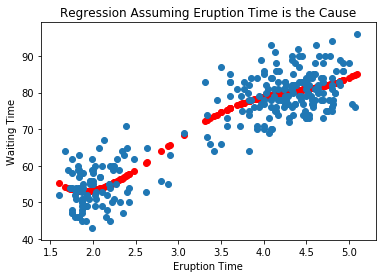
\includegraphics[scale=0.451]{erup_time1.png}
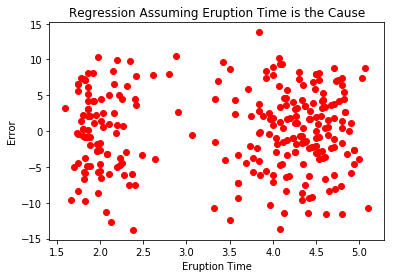
\includegraphics[scale=0.451]{erup_time2.png}
\end{floatrow}
\caption{رگرسیون با فرض اینکه زمان فوران کنونی علّت فاصله‌ی زمانی تا فوران بعدی است.}
\label{erup}
\end{figure}

\begin{figure}[h]
\begin{floatrow}
\centering
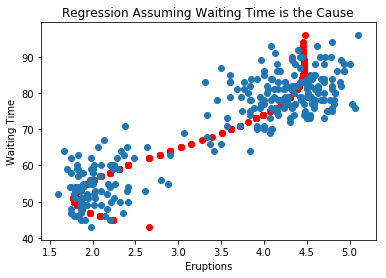
\includegraphics[scale=0.451]{waiting_time1.png}
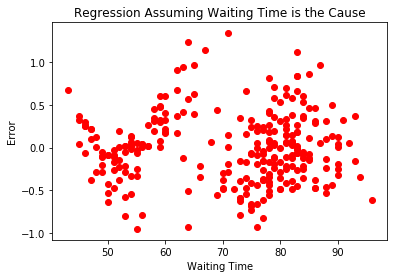
\includegraphics[scale=0.451]{waiting_time2.png}
\end{floatrow}
\caption{رگرسیون با فرض اینکه فاصله‌ی زمانی تا فوران بعدی علّت زمان فوران کنونی است.}
\label{wait}
\end{figure}
با این کار و انجام آزمون فرضیه‌ی \lr{HSIC}، متوجه می‌شویم با فرض 
\textbf{«زمان فوران کنونی علّت فاصله‌ی زمانی تا فوران بعدی است» }
زیرا همان‌طور که در شکل \eqref{erup} دیده‌ می‌شود، بعد از رگرسیون فاصله‌ی زمانی تا فوران بعدی بر حسب طول زمان فوران فعلی، مقدار residue این رگرسوراز فاصله‌ زمانی فوران فعلی مستقل است. این موضوع تا حدی بدیهی است زیرا فوران بعدی، بعد از فوران فعلی رخ داده و نمی‌تواند تاثیر علّی بر فوران فعلی داشته باشد.

\subsubsection{دیتاست صدف}
در این دیتاست قصد داریم جهت علّی بین طول این نوع صدف و تعداد حلقه‌های آن را پیدا کردیم. می‌دانیم که تعداد حلقه‌ها رابطه‌ای تقریباً غیرتصادفی با سن  صدف دارد. از نظر شهودی،‌ سن صدف(یا به عبارتی تعداد حلقه‌ها) علّت طول صدف است. در این بخش این موضوع را به کمک دیتای داده‌شده تایید می‌کنیم.
یک بار با فرض سن صدف(یا به عباری تعداد حلقه‌ها) علّت طول صدف، الگوریتم را اجر می‌کنیم. شکل 
\eqref{cor}
نتایج این کار هستند. شکل 
\eqref{wrong}
نیز نتایج اجرای الگوریتم با فرض طول صدف علّت تعداد حلقه‌ها (یا به عبارتی سن صدف) هستند.
\begin{figure}[h!]
\centering
\begin{floatrow}
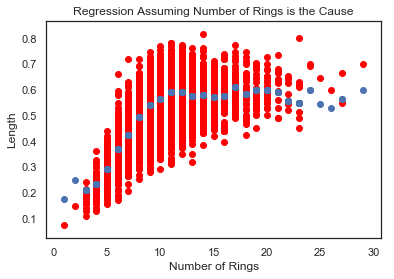
\includegraphics[scale=0.4]{aba_for1.png}
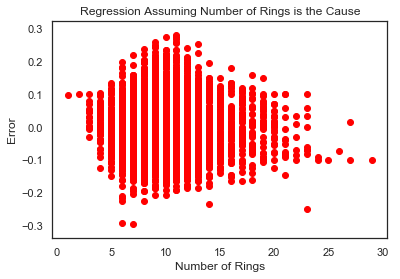
\includegraphics[scale=0.4]{aba_for2.png}
\end{floatrow}
\caption{ سن صدف(یا به عباری تعداد حلقه‌ها) علّت طول صدف}
\label{cor}
\end{figure}
\begin{figure}[h!]
\centering
\begin{floatrow}
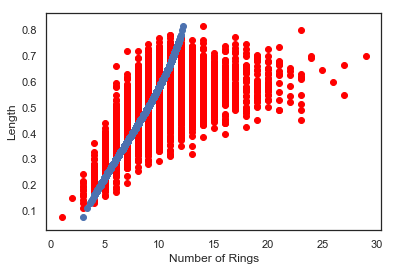
\includegraphics[scale=0.4]{aba_back1.png}
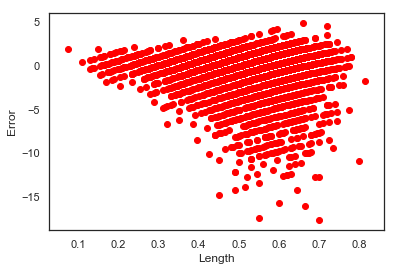
\includegraphics[scale=0.4]{aba_back2.png}
\end{floatrow}
\caption{طول صدف علّت تعداد حلقه‌ها (یا به عبارتی سن صدف)!}
\label{wrong}
\end{figure}
با توجه این نتایج و اعمال آزمون استقلال و همچنین با توجه به نمودارهای residue بر حسب متغییر علّت فرض شده، فرض ما مبنی بر اینکه
\textbf{سن صدف(یا به عباری تعداد حلقه‌ها) علّت طول صدف}
تایید می‌شود. 
%%%%%%%%%%%%%%%%%%%%%%%%%%%%%%%%%%%%%%%%%	
\newpage
\section{سوال دو}
می‌دانیم داده‌های این سوال از یک SCM تولید شده‌اند و اسکلت گراف این SCM در شکل روبروآمده است. حال سعی می‌کنیم با چند بار تکرار فرایندی که در سوال قبلی طی شد، در این سوال نیز جهت‌‌های درست گراف را تشخیص دهیم.  این کار را در چند مرحله انجام می‌دهیم. یعنی با فرض‌های مختلف علّیت، رگرسیون انجام داده و چک می‌کنیم که آیا residue این رگرسیون مستقل از علت‌های مفروض هست یا خیر. در جهت درست علیّت این شرط برقرار است.

\begin{figure}[h]
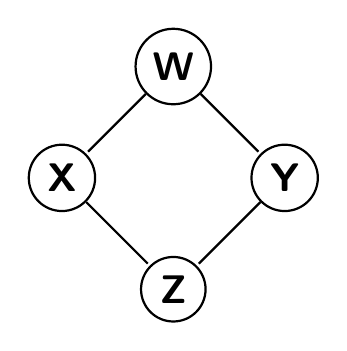
\begin{tikzpicture}[-,>=stealth',shorten >=1pt,auto,node distance=2cm,
thick,main node/.style={circle,draw,font=\sffamily\Large\bfseries}]
\node[main node] (w) {W};
\node[main node] (x) [below left of=w] {X};
\node[main node] (z) [below right of=x] {Z};
\node[main node] (y) [below right of=w] {Y};
\path[every node/.style={font=\sffamily\small}]
(w) edge node [left] {} (x)
(w) edge node [left] {} (y)
(y) edge node [left] {} (z)
(x) edge node [left] {} (z);
\end{tikzpicture}
\caption{اسکلت گراف مربوط به داده‌ها}
\label{skeleton}
\end{figure}
\vspace{0.1cm}
\begin{itemize}
\item	\textbf{ تعیین جهت یال‌های متصل به Z}	
در صورتی که فرض کنیم هر دو یال به این راس وارد می‌شود و رگرسیون
$z = \hat{f} (x, y) + \epsilon$
را حساب کنیم، دیده‌می‌شود که داریم:
$$\epsilon \bigCI X, \; \;\; \epsilon \bigCI Y$$
که این نشان می‌دهد این، جهت درست علیّت است. با فرض‌های دیگر، نتایجی مخالف انتظارمان از جهت درست علیّت بر خواهیم داشت.
در شکل
\eqref{forward1}
فرض شده است که $X \rightarrow Z \leftarrow Y$	و در شکل 
\eqref{back1}
فرض شده 
$X \rightarrow Z \rightarrow Y$.
دیده می‌شود در تمام حالت به جز شکل
\eqref{forward1}
تست‌های استقلال نتایجی سازگار با گراف ندارند و بنابراین حالت 
\eqref{forward1}
را به عنوان حالت صحیح می‌پذیریم.

\begin{figure}[h]
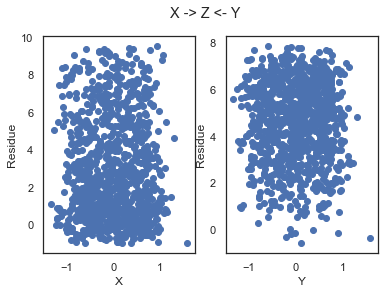
\includegraphics[scale=0.455]{b1.png}
\caption{
مقدار Residueی
$Z = \hat{f}(X,Y)$
بر حسب X و Y با فرض 
$X \rightarrow Z \leftarrow Y$	
}
\label{forward1}
\end{figure}

\begin{figure}[h]
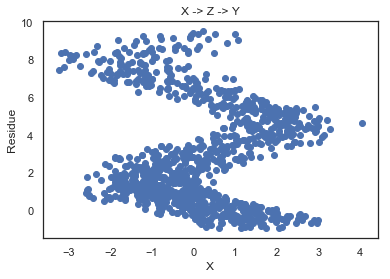
\includegraphics[scale=0.455]{b2.png}
\caption{
مقدار  Residue ی
$Z = \hat{f}(X)$
بر حسب X با فرض 
$X \rightarrow Z \rightarrow Y$	
}
\label{back1}
\end{figure}


\item	\textbf{تعیین جهت یال‌های متصل به W}	
ابتدا فرض می‌کنیم که هر دو یال از W خارج شوند. با این فرض برای X و Y داریم:
$$
\begin{cases}
X := f_1(W) + N_x\\
Y := f_2(W)  + N_y
\end{cases}
W \bigCI N_x, \;\; W \bigCI N_y
$$
حال سعی می‌کنیم این SCM را بر دیتای داده شده برازش کنیم. با انجام دو رگرسیون و بررسی استقلال Residue از علّت، به نتایج زیر می‌رسیم.
\begin{figure}[h]
\centering
\begin{floatrow}
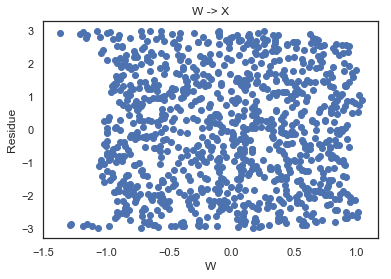
\includegraphics[scale=0.45]{WtoX.png}
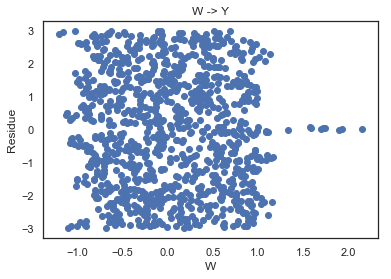
\includegraphics[scale=0.45]{WtoY.png}
\end{floatrow}
\caption{
مقدار Residue ی
$ Y=\hat{f}(W) $
و
$ X = \hat{g}(W)$
بر حسب $W$ با فرض
$ Y \leftarrow W \rightarrow X$
}
\label{Forward}
\end{figure}

این تنها حالتی است که با 
\lr{Confidence Level}
دو درصد، تمام تست‌های استقلال منجر به نتیجه‌ی مورد نظرمان می‌شوند. 
شکل
\eqref{backward}
یک فرض اشتباه است که در نهایت، Residue  ها از کمیّت‌هایی که علت ‌$W$ در نظر گرفته شده‌اند مستقل نشده است.

\begin{figure}[h]
\centering
\begin{floatrow}
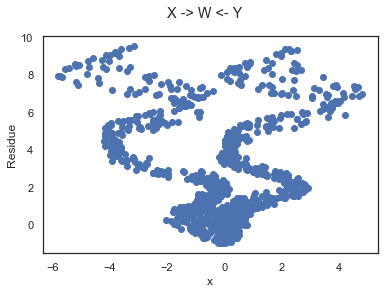
\includegraphics[scale=0.45]{back1.png}
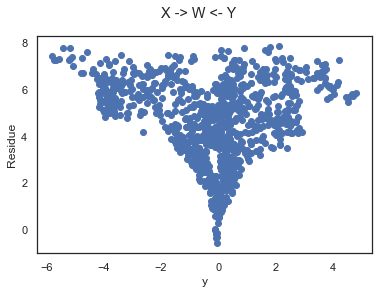
\includegraphics[scale=0.45]{back2.png}
\end{floatrow}

\caption{
مقدار Residue
$W = \hat{f}(X, Y)$
بر حسب $X$ و $Y$ با فرض 
$Y \rightarrow W \leftarrow X$
}
\label{backward}
\end{figure}
\end{itemize}

به طور کلی، ایده‌ی ما در این سوال این بود که برای راس‌ها جهت‌های مختلف فرض کرده و سپس با انجام رگرسیون‌های مربوطه و بررسی روابط استقلال، صحت جهت انتخاب شده را بررسی کنیم. در نهایت با توجه به موارد مطرح شده، گراف زیر را به عنوان یافته‌ی خود اعلام می‌کنیم.
\begin{figure}[h]
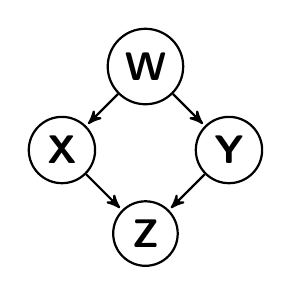
\begin{tikzpicture}[->,>=stealth',shorten >=1pt,auto,node distance=1.5cm,
thick,main node/.style={circle,draw,font=\sffamily\Large\bfseries}]
\node[main node] (w) {W};
\node[main node] (x) [below left of=w] {X};
\node[main node] (z) [below right of=x] {Z};
\node[main node] (y) [below right of=w] {Y};
\path[every node/.style={font=\sffamily\small}]
(w) edge node [left] {} (x)
(w) edge node [left] {} (y)
(y) edge node [left] {} (z)
(x) edge node [left] {} (z);
\end{tikzpicture}
\caption{گراف نهایی}
\label{final}
\end{figure}
\end{document}